\documentclass[cn,table]{elegantbook}

\usepackage{tikz}
\usepackage{graphicx}
\usepackage{subcaption}
\usepackage[ruled,linesnumbered,vlined]{algorithm2e}
\usepackage{hyperref}
\usepackage{listings}
\usepackage{interval}
\usepackage{xcolor}
\usepackage{ulem}
\usepackage{wrapfig}

\intervalconfig{%
	soft open fences,
}

\def\figureautorefname{图}
\def\sectionautorefname{小节}

\SetAlgorithmName{算法}{算法}{算法索引}

\renewcommand*{\lstlistingname}{代码}

\title{何老师算法课笔记}
\subtitle{Always be patient, sharp and diligent.}
\author{计卓1801全体}
\institute{华中科技大学}
\date{\zhtoday}
\version{1.6.2}
\logo{logo.png}
\cover{cover.png}

\begin{document}
\maketitle
\tableofcontents
\pagenumbering{arabic}

% add your code here
% \input{src/example.tex}
\input{src/Ln1-AsymptoticOrderGrowth.tex}
\input{src/Tiling-Problem.tex}
\input{src/stable-matching.tex}
\input{src/Ln9-NearestPoints.tex}
\input{src/Ln11-LargeIntegerMultiplication.tex}
\input{src/dynamic-programming-1.tex}
\input{src/Network-flows.tex}
\chapter{网络流应用之图像分割}

\centering{本章简单介绍网络流在图像分割上的应用。}
{\centering 本章简单介绍网络流在图像分割上的应用。}

\begin{definition}{背景知识}{}
	图像是可以看作由一个个像素组成的巨大图, 将像素一一用边连接起来, 则这些像素点会成为这个巨大图网络的顶点.
	一个图由前景和背景组成, 假设顶点上的值用 $a_i$ 表示, $ 0 \leq a_i \leq 1 $,  $a_i$ 趋近于 0 表示 $a_i$ 为图的背景, $a_i$ 趋近于 1 表示 $a_i$ 为图的前景, 并且设所有属于前景的顶点 $a_i$ 构成集合 A, 所有属于背景的顶点 $a_j$ 构成集合 B.
	假设边上的值用 $w_{ij}$ 表示, $w_{ij}$ 设为边的惩罚值, $w_{ij}$ 趋向于 0 表示“分离” (即 $w_{ij}$ 连接的两个点分别属于前景和背景), $w_{ij}$ 趋向于 1 表示“在一起” (即 $w_{ij}$ 连接的两个点都属于前景或者背景)
	设总的惩罚值为 $ A = \min\left(\sum_{i \epsilon B}a_i +  \sum_{i \epsilon A}(1 - a_j) + \sum_{i \epsilon A, j \epsilon B}w_{ij} \right) $
\end{definition}


\section{问题实例}
\subsection{问题描述}
\begin{itemize}
	\item 对于下面这个图,利用网络流求解该图前景和背景的最大可能
\end{itemize}

\begin{figure}[htb]
	\centering
	\includegraphics[scale=0.8]{image/Image-segmentation2.png}
	\caption{图片前景背景识别}\label{fig:image-seg-1}
\end{figure}

\subsection{思路描述}
\begin{itemize}
	\item 图形切割算法通过向图 G (V,E) 添加 S 点和 T 点,将图中所有的顶点,与 S 和 T 建立边,
	      如果一个点与 S 相连,则对应边的权值为该点的值 $a_i$, 如果一个点与 T 相连,则对应边的权值为1减去该点的值 $ 1 - a_j $。
	      可以得到下面这个图:
\end{itemize}

\begin{figure}[htb]
	\centering
	\includegraphics[height=4.5cm]{image/Image-segmentation3.png}
	\caption{图片前景背景识别}\label{fig:image-seg-2}
\end{figure}

\begin{itemize}
	\item   根据最大流最小割, 可以得到得到二分图的最大匹配, 可以得到集合A和B, 保证总的惩罚值 $ A = \min\left(\sum_{i \epsilon B}a_i +  \sum_{i \epsilon A}(1 - a_j) + \sum_{i \epsilon A, j \epsilon B}w_{ij} \right) $ 最小,
	      最小为 $(0.2 + 0.1) + (1 - 0.9) + (1 - 0.8) + 0.3 + 0.3 = 1.2 $, 而 A 和 B 分别对应图的前景和背景。
\end{itemize}

\section{问题扩展}
\begin{itemize}
	\item 假如一个图的前景不是一个整体,
	      而是有两个分开的部分,比如两只在两个不同位置的猫在一个图中。
	      这样一个算法能否将图像上的前景和背景分开?
\end{itemize}

\begin{figure}[htb]
	\centering
	\includegraphics[scale=0.6]{image/Image-segmentation1.png}
	\caption{图片前景背景识别}\label{fig:image-seg-3}
\end{figure}

\chapter{图算法之最小生成树}

\begin{introduction}
	\item 问题概述
	\item Prim算法
	\item Kruskal算法
\end{introduction}

\section{概述}
给定一张边带权的无向图G=(V, E),其中V表示图中点的集合,E表示图中边的集合,n=|V|,m=|E|。
由V中的全部n个顶点和E中n-1条边构成的无向连通子图被称为G的一棵生成树,其中边的权值之和最小的生成树被称为无向图G的最小生成树。

最小生成树最为经典的两个算法分别是Prim算法和Kruskal算法。本节将首先讨论这两个算法的执行过程。

\section{基本概念}
在深入探讨之前,还需明白一些定义:

\begin{definition}{path}{path}
	A path is a sequence of edges which connects a sequence of nodes.
\end{definition}

\begin{definition}{cycle}{cycle}
	A cycle is a path with no repeated nodes or edges other than the
starting and ending nodes.
\end{definition}

可以借助\autoref{fig:path-cycle}理解path以及cycle的概念。

\begin{figure}[hbt]
	\centering
	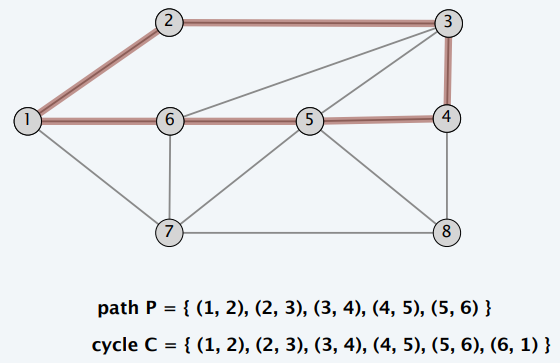
\includegraphics[scale=0.5]{image/pathcycle.png}
	\caption{具体例子说明path和cycle}\label{fig:path-cycle}
\end{figure}

\begin{definition}{cut}{MSTcut}
	A cut is a partition of the nodes into two nonempty subsets S and V / S.
\end{definition}

\begin{definition}{cutset}{MSTcutset}
	The cutset of a cut S is the set of edges with exactly one endpoint in S.
\end{definition}

可以借助\autoref{fig:cut-cutset}理解cut以及cutset的概念。

\begin{figure}[hbt]
	\centering
	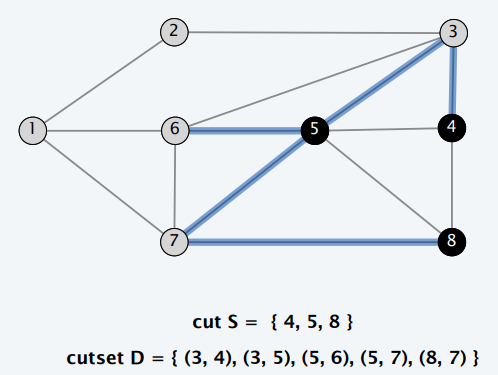
\includegraphics[scale=0.5]{image/cutcutset.png}
	\caption{具体例子说明cut与cutset}\label{fig:cut-cutset}
\end{figure}

\begin{theorem}{}{cycle-cutset-theorem}
	A cycle and a cutset intersect in an even number of edges.
\end{theorem}

可以借助\autoref{fig:cycle-cutset}理解\autoref{cycle-cutset-theorem}。

\begin{figure}[hbt]
	\centering
	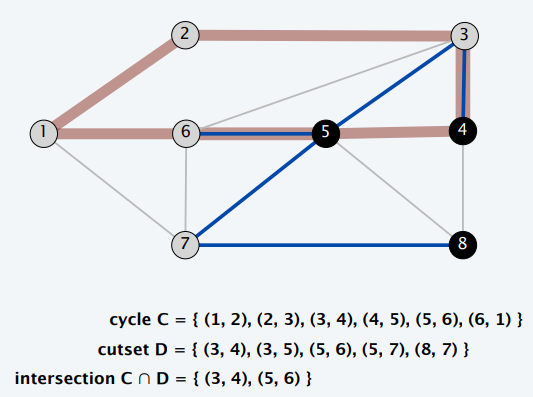
\includegraphics[scale=0.5]{image/cyclecutset.png}
	\caption{cycle、cutset的性质}\label{fig:cycle-cutset}
\end{figure}

\begin{definition}{生成树}{ST}
Let H = (V, T) be a subgraph of an undirected graph G = (V, E).
H is a spanning tree of G if H is both acyclic and connected.
\end{definition}

一个生成树的例子如\autoref{fig:exampleofST}所示。

\begin{figure}[hbt]
	\centering
	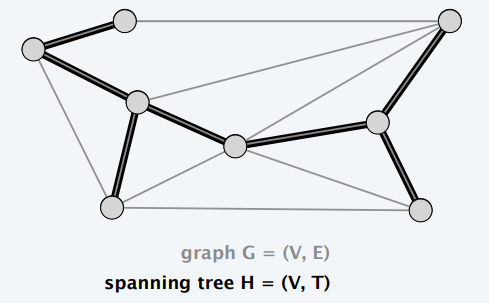
\includegraphics[scale=0.5]{image/exampleofST.png}
	\caption{生成树的例子}\label{fig:exampleofST}
\end{figure}

\begin{theorem}{}{ST-theorem}
	如果H = (V, T)是一个无向图G = (V, E)的子图,那么,以下各条件等价:
	\begin{enumerate}
		\item H是G的一棵生成树
		\item H是无环且连通的
		\item H是连通的并且有 V – 1条边
		\item H是无环的并且有 V – 1条边
		\item 任意拿掉H的一条边,就不再使其连通
		\item 任意增加一条边,则H就会构成环
	\end{enumerate}

\end{theorem}

\begin{definition}{最小生成树}{MST}
	Given a connected, undirected graph G = (V, E) with edge costs $c_e$,
a minimum spanning tree (V, T) is a spanning tree of G such that the sum
of the edge costs in T is minimized.
\end{definition}

一个生成树的例子如\autoref{fig:exampleofMST}所示。

\begin{figure}[hbt]
	\centering
	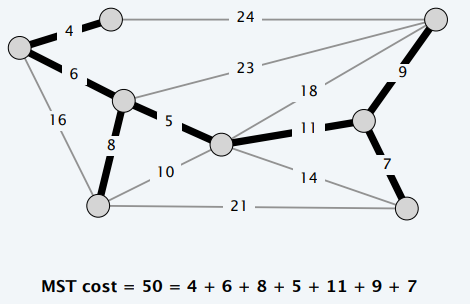
\includegraphics[scale=0.5]{image/exampleofMST.png}
	\caption{生成树的例子}\label{fig:exampleofMST}
\end{figure}

\begin{theorem}{Cayley’s theorem}{Cayley-theorem}
	The complete graph on n nodes has $n^(n–2)$ spanning trees
\end{theorem}

最小生成树是一个基础却有着十分广泛的应用的问题,之后的\autoref{sec:prim}和\autoref{sec:kruskal}
将分别介绍求解最小生成树的Prim算法和Kruskal算法。

\section{Prim算法}\label{sec:prim}
\subsection{算法描述与演示}
\begin{algorithm}
	\DontPrintSemicolon
	\KwIn{Graph G}
	\KwResult{MST of Graph G}
	\Begin{
		$S \leftarrow \{ s \} $ for any node s,$T \leftarrow \emptyset$;\\
		\For{$|T| < n-1$}{
			Add to T a min-weight edge with exactly one endpoint in S;\\
			Add the other endpoint to S;\\
		}
		Return T ;\\
	}
	\caption{Prim}\label{alg:Prim}
\end{algorithm}

算法执行流程如\autoref{fig:Prim}所示。

\begin{figure}[hbt]
	\centering
	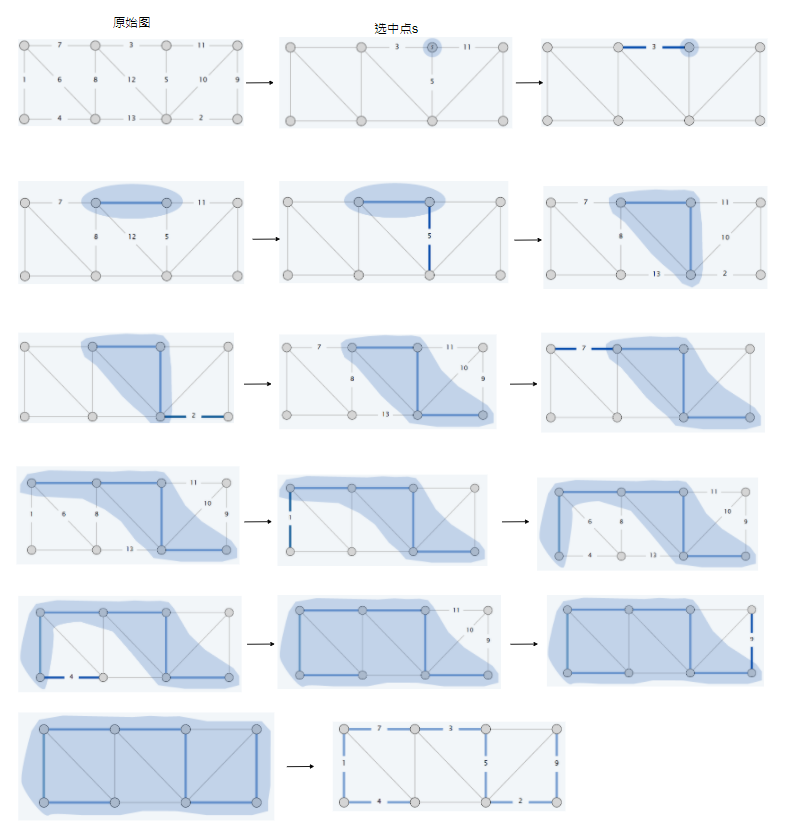
\includegraphics[scale=0.5]{image/prim.png}
	\caption{Prim算法的执行流程}\label{fig:Prim}
\end{figure}

\subsection{算法正确性证明}
\noindent记图G是一个连通图,Y是对p使用prim算法得到的一棵生成树,$Y_1$是p的一棵最小生成树
\begin{enumerate}
	\item 若Y=$Y_1$,显然prim算法是正确的
	\item 若Y≠$Y_1$,可进行如下推导:

	a)Y中有$n( n \geq 1 )$条边不存在于$Y_1$中,在构建Y的过程中,第一次遇到这样的一条边时(以e表示),
	则e的一个端点u落在V内(V是之前的prim运算得到的一个子顶点集),另一个端点v落在V外
	
	b)$Y_1$是连通的,故$Y_1$中存在u到v的一条的路径,此路径上必然存在一条边f,它的一个端点落在V内,另一个端点落在V外
	
	c)把e加入$Y_1$,去掉f,$Y_1$仍然连通,根据prim算法,权值$W(f) \geq W(e)$,否则e不会被选入V,
	如果$W(f)>W(e)$,新构建的树的权值和会比$Y_1$小,而$Y_1$是最小生成树,因此$W(f)>W(e)$不成立,得$W(f)=W(e)$
	
	d)对每一条类似e的边,重复过程c),最终Y和重新构建的的$Y_1$拥有的边完全一致,
	新构建的$Y_1$也是最小生成树,因此Y也是最小生成树,证明prim算法正确
\end{enumerate}

\subsection{算法复杂度}
普通堆优化的 Prim 算法复杂度为 $O(mlogn)$,而斐波那契堆优化的 Prim 算法
能达到 $O(m+nlogn)$

\section{Kruskal算法}\label{sec:kruskal}
\subsection{算法描述与演示}
\begin{algorithm}
	\DontPrintSemicolon
	\KwIn{Graph G}
	\KwResult{MST of Graph G}
	\Begin{
		$T \leftarrow \emptyset$;\\
		$S \leftarrow$sort edges by weight;\\
		\While{$e \in S$}{
			\If{$T \cup \{ e \}$ no cycle}{
				$T = T \cup \{ e \};$
			}
			\If{$|T| < n-1$}{
				Return T ;\\
			}
		}
	}
	\caption{kruskal}\label{alg:kruskal}
\end{algorithm}

算法执行流程如\autoref{fig:kruskal}所示。

\begin{figure}[hbt]
	\centering
	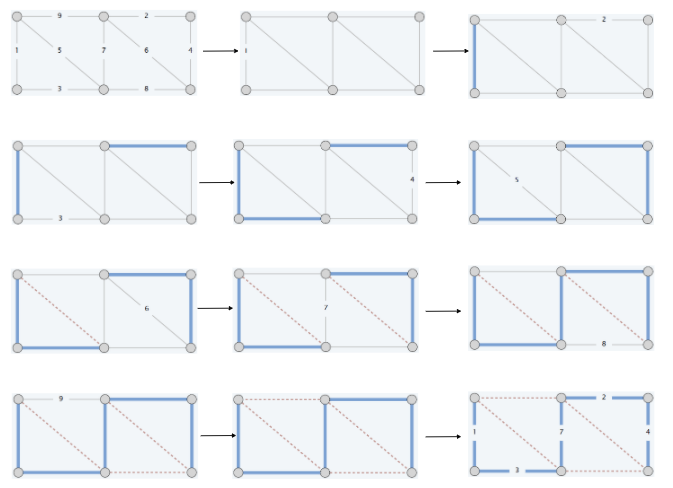
\includegraphics[scale=0.5]{image/kruskal.png}
	\caption{Kruskal算法的执行流程}\label{fig:kruskal}
\end{figure}

\subsection{算法正确性证明}
Kruskal算法每次会向T添加一条最小权重的边,并且不能形成环.
对于一棵树而言, 如果有K个节点, 则必然有K-1条边
我们要证明的问题其实是连续添加的边E(l) l=0,1,2...K-1 是一颗最小生成树MST的子集.

对于基本情况, 如果I = 0, 此时为空集,满足条件;

现在我们假设对 $0 \leq m < K-1$, E(m) 已经满足条件,是$T_1$的子集. 我们来看 E(m+1)的情况,
有E(m+1) = E(m) + {e}, e为算法当前新增的最小权重边.此时分两种情况:

\begin{enumerate}
	\item 如果{e}是$T_1$的子集,那么问题解决;
	\item 如果{e}不是$T_1$的子集, 那么我们要证明 E(m+1) 属于一颗其他的MST子集:

	因为{e}不是$T_1$的边, 所以 $T_1$ + {e} 必然有环C(性质1), 同时 E(m) 属于 $T_1$ ,
	那么在环C上必然有一个{e'} 不属于E(m) (因为如果属于E(m)的化, 那么算法当前选择的{e}会导致一个环, 与性质1违背).
	
	现在我们定义$T_2$ = $T_1$ + {e} - {e'}, 又因为E(m+1) = E(m) + {e} 所以 E(m+1) 属于$T_2$的子集.$T_2$是一颗MST.
	
	因为{e} 和 {e'} 都不属于 E(m), 算法当前选择的是{e} 说明 $weight({e'}) \geq weight({e})$.
	所以我们看$weight(T_2) = weight(T_1) + weight({e}) - weight({e'}) \leq weight(T_1)$ .
	
	这意味着$T_1$是$T_2$的权重upper-bound, 但由于$T_1$已经是MST, 所以必然的$T_2$也是MST. 至此得证.	
\end{enumerate}

\subsection{算法复杂度分析及优化}
\begin{theorem}{}{Kruskal-theorem}
	Kruskal’s algorithm can be implemented to run in $O(m log m)$ time.
\end{theorem}

\begin{enumerate}
	\item Sort edges by cost:$O(m log m)$.
	\item Use union–find data structure to dynamically maintain connected components:$O(m \alpha (n))$.
\end{enumerate}

\begin{remark}
	$\alpha (n)$是反阿克曼函数,阿克曼函数 $A(m,n)$ 增长极快,其反函数几乎是常数。
\end{remark}

下面将简要介绍并查集(union–find data structure)有关内容。
\subsection{并查集}
在计算机科学中,并查集是一种树型的数据结构,用于处理一些不交集(Disjoint Sets)的合并及查询问题。
有一个联合-查找算法(union-find algorithm)定义了两个用于此数据结构的操作:

Find:确定元素属于哪一个子集。它可以被用来确定两个元素是否属于同一子集。

Union:将两个子集合并成同一个集合。

在并查集森林中,每个集合的代表即是集合的根节点。“查找”根据其父节点的引用向根行进直到到底树根。
“联合”将两棵树合并到一起,这通过将一棵树的根连接到另一棵树的根。实现这样操作的一种方法是

\begin{lstlisting}
function MakeSet(x)
     x.parent := x

function Find(x)
     if x.parent == x
        return x
     else
        return Find(x.parent)

function Union(x, y)
     xRoot := Find(x)
     yRoot := Find(y)
     xRoot.parent := yRoot
\end{lstlisting}

这是并查集森林的最基础的表示方法,这个方法不会比链表法好,这是因为创建的树可能会严重不平衡;然而,可以用两种办法优化。

第一种方法,称为“按秩合并”,即总是将更小的树连接至更大的树上。因为影响运行时间的是树的深度,
更小的树添加到更深的树的根上将不会增加秩除非它们的秩相同。在这个算法中,术语“秩”替代了“深度”,因为同时应用了路径压缩时秩将不会与高度相同。

第二个优化,称为“路径压缩”,是一种在执行“查找”时扁平化树结构的方法。关键在于在路径上的每个节点都可以直接连接到根上;
他们都有同样的表示方法。为了达到这样的效果,Find递归地经过树,改变每一个节点的引用到根节点。得到的树将更加扁平。

\chapter{最小生成树其他算法}

\begin{introduction}
	\item red/blue算法
	\item Boruvka算法
\end{introduction}

本章将介绍求解最小生成树的red/blue算法和Boruvka算法。

\section{red/blue算法}

\subsection{基本概念}
下面给出red/blue算法有关内容的定义
\begin{definition}{割(cut)}{cut}
	S$\in$V,S$\neq \emptyset$,点集V被划分成互补的子集S和V/S。
\end{definition}

\begin{definition}{割边集(cutset)}{cutset}
    对于图G的顶点集V的割X、Y,图G的边集E中连接两集合X、Y的所有边的集合叫做这个割的割边集(cutset)。
\end{definition}

\begin{definition}{Red Rule}{Red Rule}
    找到图G中不含红色边的环C,从C中未被染色的边中选出边权最大的边将其染成红色。
\end{definition}

\begin{definition}{Blue Rule}{Blue Rule}
    找到图G中不含蓝色边的割边集D,从D中未被染色的边中选出边权最小的边将其染成蓝色。
\end{definition}

\subsection{算法运行步骤}
\begin{enumerate}
	\item 初始化:对于给定的图G,将所有边标记为未染色。
	\item 在图G中同时运行Red Rule和Blue Rule (可并行运行),直到所有边均被染色为止。
	\item 图G中所有的蓝色边即为图G的最小生成树。
\end{enumerate}

算法具体执行过程如\autoref{fig:redblue}
\begin{figure}[hbt]
	\centering
	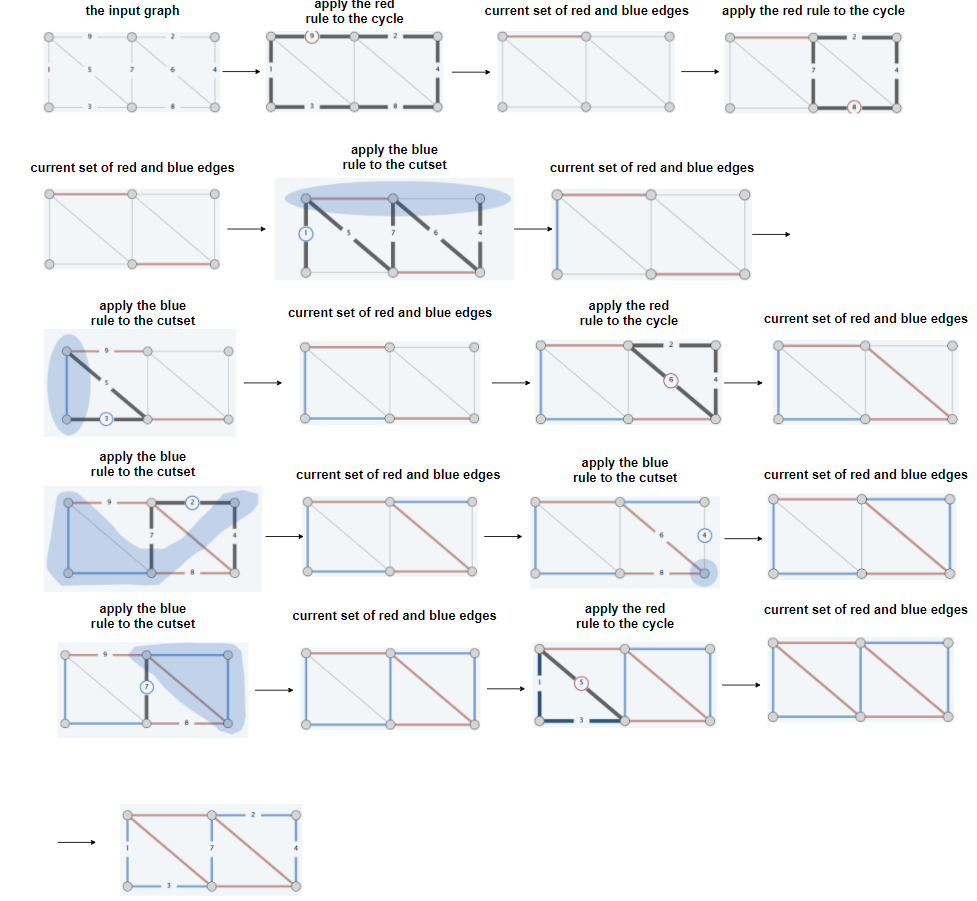
\includegraphics[scale=0.4]{image/redblue.png}
  \caption{red/blue算法执行过程图解}\label{fig:redblue}
\end{figure}

\subsection{算法正确性证明}\label{sec:redblue-proof}
\begin{enumerate}
	\item 最优性:Blue Rule染色所得边为最小边

对于图G中的一个割边集D及D中边权最小的边minEdge,如果在Blue Rule运行过程中被染色的是割边集D的其他边biggerEdge,
则可以在最后得到的MST中将biggerEdge从中删除然后将minEdge加入到MST中,可以得到更小的最小生成树。产生矛盾。所以Blue Rule染色所得边为最小边。
\item 合法性:算法所得所有蓝边为无环连通图

由于Blue Rule可知每次选边都不会成环。下证所得为连通图,假设最后所得所有蓝边构成的图不连通或仍然有点未被蓝边连接。

对于第一种情况,则任选某一蓝边的一个顶点并从该顶点开始的所有能通过蓝边的顶点记为集合X,
S与V/S构成图G的一个割,由Red Rule中所选环C不含红色边可知其割边集不可能全部被染成红色,则说明一定有未染色的边,再应用一次Blue Rule即可增大S的点的个数,
重复上述过程直到S=E;对于第二种情况,由于孤立点必不可能在某个环中,所以连接该点的边一定不会被Red Rule染成红色,所以此时应用一次Blue Rule即可使得该点被蓝边连接。综上,算法所得所有蓝边为连通图
\end{enumerate}

\section{Boruvka算法}
\subsection{算法运行步骤}
\begin{enumerate}
	\item 初始化:对于给定的图G,将所有边标记为未染色;将每个顶点作为一个连通块。
	\item 对于所有蓝边连成的连通块应用Blue Rule并将所有Blue Rule选中的边染成蓝色,直到只有一个连通块。
	\item 最后得到的蓝边连成的连通块即为图G的最小生成树。
\end{enumerate}

算法具体执行过程如\autoref{fig:boruvka}
\begin{figure}[h]
	\centering
	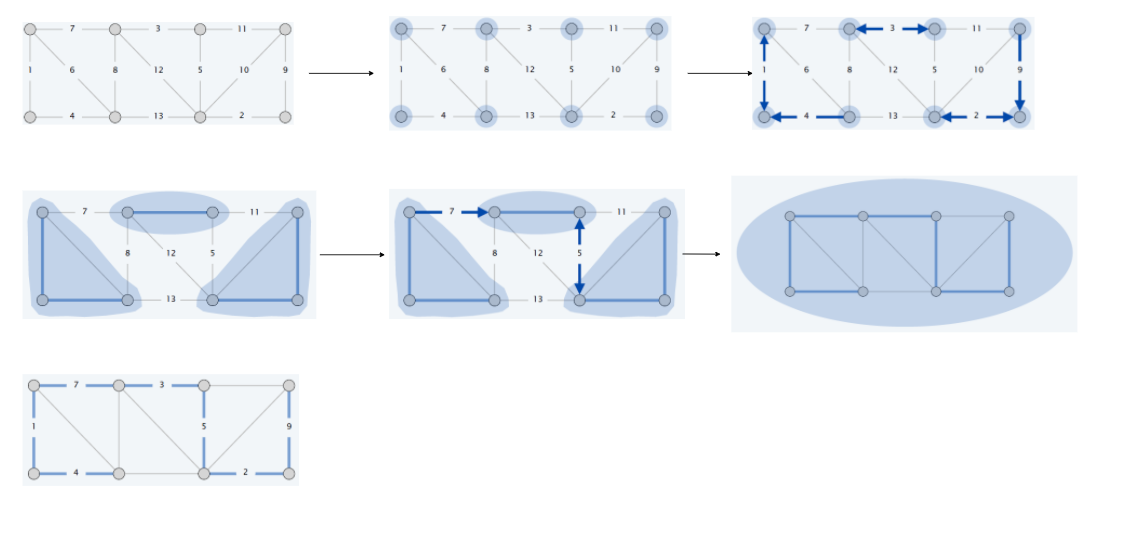
\includegraphics[scale=0.4]{image/boruvka.png}
  \caption{boruvka算法执行过程图解}\label{fig:boruvka}
\end{figure}

算法复杂度分析:每次应用Blue Rule后连通块数量至少减半,每次都要遍历所有边,所以算法串行时间复杂度为O(E$\log V$),并行时间复杂度为O(E)。

\subsection{算法正确性证明}
\begin{enumerate}
	\item 最优性:根据~\ref{sec:redblue-proof}中的证明:Blue Rule染色所得边为最小边。
	\item 合法性:一定不会构成环。如果存在环说明一个点的最小连边有两个,与Blue Rule矛盾。
\end{enumerate}


\bibliography{ref.bib}
\end{document}
